\subsection{Definiciones previas}

% IR AGREGANDO EN ORDEN ALFABÉTICO

\subsubsection*{Gamificación}

Comúnmente, la gamificación se define como un proceso intencionado de transformación de cualquier actividad, sistema, servicio, producto o estructura organizativa en uno que ofrece experiencias positivas experiencias positivas, habilidades y prácticas similares a las similares a las que ofrecen los juegos, y a menudo se denomina experiencia lúdica. Esto se hace comúnmente, pero opcionalmente, con la intención de facilitar cambios en los comportamientos o procesos cognitivos \cite{gamificationRef}. Como las principales inspiraciones de la gamificación son los juegos y el juego, la gamificación se suele llevar a cabo empleando el diseño del juego (por ejemplo, los elementos de las estructuras de objetivos, la mecánica de retroalimentación, la narrativa y el diseño visual), las estructuras sociales (por ejemplo, el diseño visual, la accesibilidad), competencias sociales (por ejemplo, competencia y colaboración), juegos de rol y tecnologías de inmersión como la realidad virtual y la realidad aumentada.


\subsubsection*{Estrategias de Gamificación}

Las estrategias de gamificación contribuyen al desarrollo, tanto de competencias específicas como transversales en procesos de enseñanza-aprendizaje; se utilizan para promover conductas que despierten el interés de los estudiantes por aprender \cite{Gonzalez}. Los elementos considerados para la elaboración de la estrategia de gamificación se clasifican en tres categorías: dinámicas, mecánicas y componentes \cite{Gee}.

    \begin{itemize}
        \item Las dinámicas se refieren al motor que permite el funcionamiento de la estrategia. Son los factores generales en los que debe estar centrado un sistema de gamificación. Están directamente relacionados con el desempeño favorable que se espera del participante \cite{guevara}.
        
        \item Las mecánicas se relacionan con la motivación y el comportamiento de los estudiantes. Representan las reglas y las recompensas que hacen que los juegos se conviertan en desafíos, provocando emociones que un sistema gamificado busca generar en los participantes. Para lograrlo se recurre a elementos como: retos, desafíos, premios, puntos, clasificaciones, niveles y regalos \cite{guevara}.
        
        \item Los componentes son las herramientas y los recursos que se utilizan para elaborar las actividades que se desarrollan en la practica de la gamificación \cite{werbach}. La figura \ref{Piramide} muestra la pirámide de los elementos de gamificación:
        
        \vspace{2mm}
        \begin{minipage}{0.9\textwidth}
        \centering
        \captionof{figure}[{Pirámide Elementos de Gamificación}]{ Pirámide Elementos de Gamificación }
        \label{Piramide}
         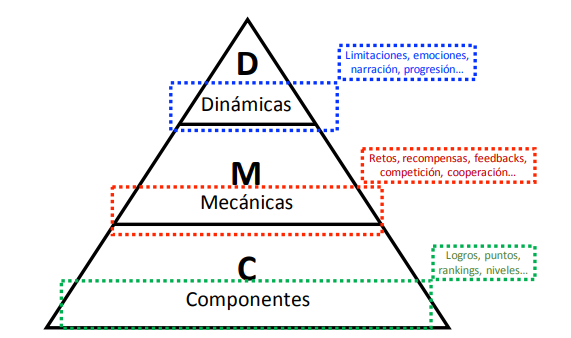
\includegraphics[width=0.6\textwidth]{Images/piramide}
          %esto es lo nuevo que agregue

        \fnote{Nota. \textup{Fuente: Adaptado de Werbach & Hunter.}}
        \end{minipage}
    \end{itemize}


\subsubsection*{Ingeniería Web}

Basada en principios científicos y de ingeniería, la Ingeniería Web pretende establecer enfoques sistemáticos para desarrollar, desplegar y mantener con éxito sistemas de alta calidad basados en la Web. También incorpora principios y prácticas de ingeniería de software bien conocidos de diversas áreas, como la interacción persona-ordenador (HCI), el análisis y el diseño de sistemas, la ingeniería de requisitos, la ingeniería hipermedia, las estructuras de datos, las pruebas y la gestión de proyectos, así como las ciencias sociales, las artes y el diseño gráfico \cite{webEngineer}.

\subsubsection*{Plan de Negocios}

Un plan de negocio como un instrumento de gestión de la empresa que sirve de guía para el emprendedor o empresario implemente un negocio. Es decir, el plan de negocio, es un instrumento de planificación que permite comunicar una idea de negocio para gestionar su financiamiento \cite{villaran}.

\subsubsection*{Profesionales en TI}

En Colombia, las carreras relacionadas con Tecnologías de Información están relacionadas principalmente con la Ingeniería de Sistemas, Telemática y afines. La Ingeniería de Sistemas como disciplina o carrera profesional representa el 66\% de la oferta académica en Colombia. Los profesionales de esta área tienen la capacidad de participar y contribuir en el análisis, comprensión y solución de problemas a través de la tecnología en diferentes áreas y sectores de la economía \cite{MinticProf}.

\subsubsection*{Pruebas Técnicas}

Las pruebas de conocimiento o habilidades específicas pretenden comprobar las destrezas técnicas y el grado de habilidad para la puesta en práctica de los conocimientos teóricos y experiencia que el candidato posee. Depende de cada empresa y el nivel de candidato buscado, para la aplicación, pueden ser al inicio del proceso, o a la mitad del mismo, así como la profundidad de ellas. \cite{pruebasTec} 

\subsubsection*{Reclutamiento 2.0}

Procedimientos para atraer e identificar a candidatos potencialmente calificados y capaces utilizando las posibilidades de la web a través de diferentes acciones: Publicar oportunidades para obtener postulaciones y ofrecer posibles puestos de trabajo a personas que no están buscando empleo de manera activa \cite{reclutamiento2}.

\subsubsection*{Recursos Humanos}

Los recursos humanos son un departamento dentro de las empresas en el que se gestiona todo lo relacionado con las personas que trabajan en ella. Esto incluiría desde el reclutamiento y selección de personal, contratación, onboarding o bienvenida, formación, promoción, nóminas, contratos y despidos. En definitiva, el departamento de recursos humanos debe trabajar para todas las personas que forman parte del Capital Humano y talento. Los recursos humanos son indispensables para cualquier empresa que necesite crecer y contratar a los mejores trabajadores para cada puesto \cite{recursos}

\subsubsection*{Rotación de Personal}

La Rotación de personal es la proporción de empleados que sale de una compañía en determinado periodo, por lo general de un año. La rotación de personal puede definirse como: el número de trabajadores que salen y entran, en relación con el total de una empresa, sector, nivel jerárquico, departamento o puesto \cite{rotacion}.